\documentclass[border=10pt]{standalone}
\usepackage[svgnames]{xcolor}
\usepackage{amsmath}
\usepackage{pgfplots}
\pgfplotsset{compat=newest}
\usepackage[sfdefault]{FiraSans}
\usepackage{FiraMono}
\renewcommand*\familydefault{\sfdefault}
\begin{document}
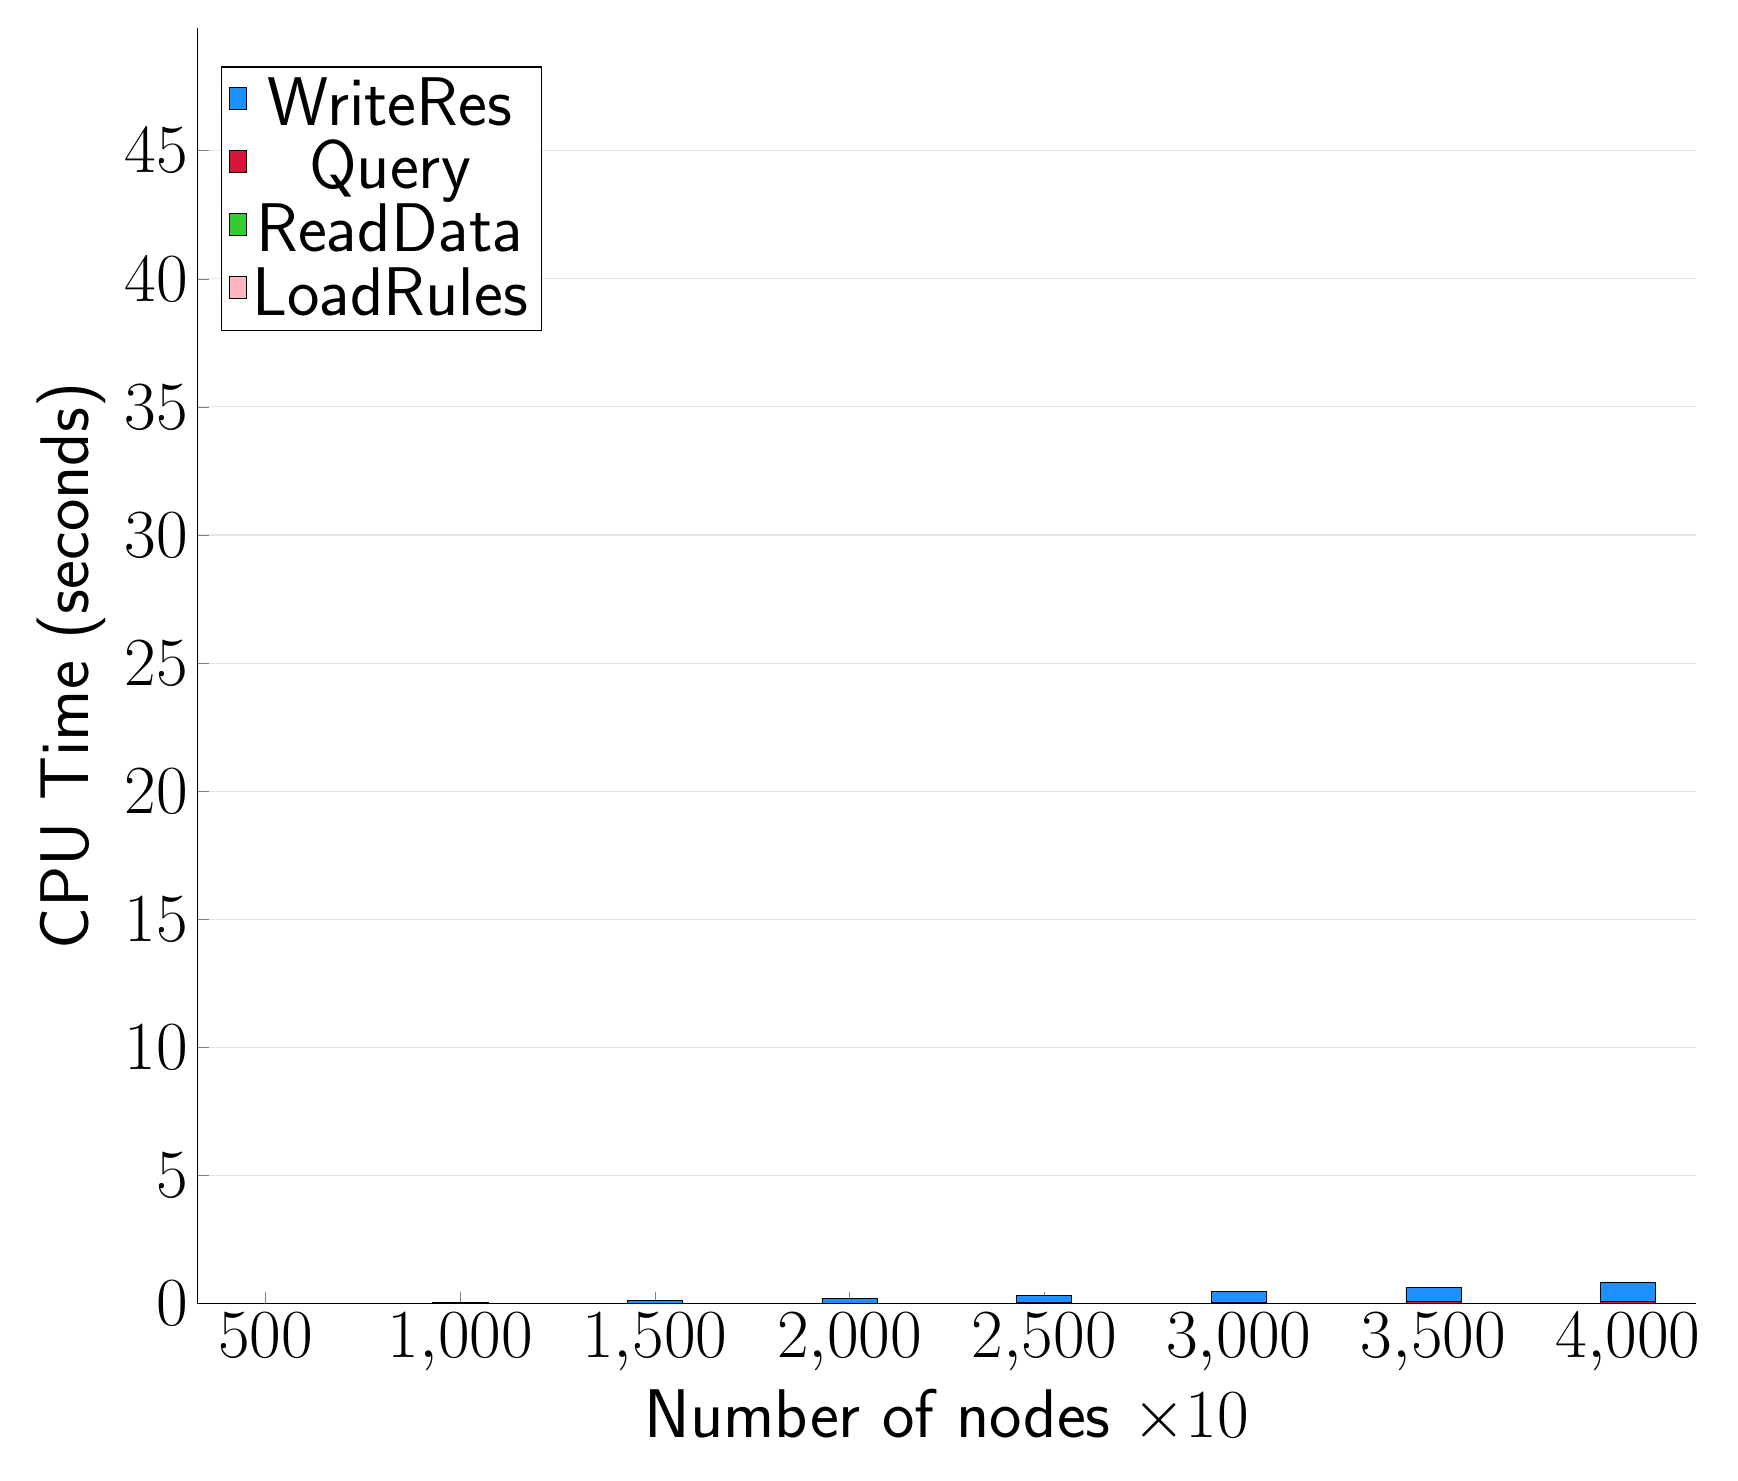
\begin{tikzpicture}
\begin{axis}[
   ybar stacked,
   width=1.7\textwidth,
   bar width=0.7cm,
   ymajorgrids, tick align=inside,
   major grid style={draw=gray!20},
   xtick=data,
   ymin=0, ymax=49.78293,
   axis x line*=bottom,
   axis y line*=left,
   enlarge x limits=0.05,
   legend style={
       at={(0.23, 0.97)},
       anchor=north east,
       legend columns=1,
       font=\Huge,
   },
   ylabel={CPU Time (seconds)},
   xlabel={Number of nodes $\times 10$},
   label style={font=\Huge},
   tick label style={font=\Huge},
]
\addlegendimage{fill=DodgerBlue, draw=black, line width=0.2pt}
\addlegendentry{WriteRes}
\addlegendimage{fill=Crimson, draw=black, line width=0.2pt}
\addlegendentry{Query}
\addlegendimage{fill=LimeGreen, draw=black, line width=0.2pt}
\addlegendentry{ReadData}
\addlegendimage{fill=LightPink, draw=black, line width=0.2pt}
\addlegendentry{LoadRules}
\addplot +[fill=LightPink, draw=black, line width=0.2pt] coordinates {
(500, 0.0006144000000000004)
(1000, 0.0006170000000000001)
(1500, 0.0006036000000000001)
(2000, 0.0006014000000000002)
(2500, 0.0006100000000000003)
(3000, 0.0006083000000000001)
(3500, 0.0006330999999999999)
(4000, 0.0006348999999999995)
};
\addplot +[fill=LimeGreen, draw=black, line width=0.2pt] coordinates {
(500, 0.0005751999999999997)
(1000, 0.001001399999999999)
(1500, 0.0014525)
(2000, 0.0019239000000000003)
(2500, 0.0023976)
(3000, 0.0028595)
(3500, 0.0032928)
(4000, 0.0037789000000000004)
};
\addplot +[fill=Crimson, draw=black, line width=0.2pt] coordinates {
(500, 0.0013463999999999998)
(1000, 0.005301599999999999)
(1500, 0.0119086)
(2000, 0.0221653)
(2500, 0.0338746)
(3000, 0.050072799999999994)
(3500, 0.0680577)
(4000, 0.0915405)
};
\addplot +[fill=DodgerBlue, draw=black, line width=0.2pt] coordinates {
(500, 0.011429)
(1000, 0.046037499999999995)
(1500, 0.10270350000000002)
(2000, 0.18078100000000003)
(2500, 0.2857507)
(3000, 0.4086659)
(3500, 0.5595814000000001)
(4000, 0.7277069)
};
\end{axis}
\end{tikzpicture}

\end{document}
